\chapter{Direct Derivation of the Height Function from the Quadratic Sequence}
\section{Introduction}

The construction of the conical helix rests on a remarkable
interplay between arithmetic and geometric structures.
The starting point is the quadratic sequence


\[
k(n)=\frac{1}{6}(2n^{2}+3n+1),
\]


whose analytic continuation is a parabola with a clearly pronounced
symmetry and a well-defined vertex. This
quadratic structure not only provides a natural ordering of the
integer function values, but simultaneously determines the
scaling and shift parameters that appear in the height component of the
helix.

The aim of this chapter is to derive the height function of the conical helix,


\[
z(\theta)=-\frac{3}{4}+\frac{3}{\pi}\theta,
\]


directly from the properties of the sequence. The derivation proceeds
without recourse to intermediate constructions and shows that both the
shift by $-\tfrac{3}{4}$ and the slope $\tfrac{3}{\pi}$
are immediate consequences of the underlying quadratic
arithmetic. The additive constant reflects the location of the
vertex of the parabola, while the slope arises from the
residue class structure modulo $6$, which enforces a linear coupling
between the angular parameter and the arithmetic progression.

This makes visible that the height component of the helix is a direct and structurally
necessary consequence of the arithmetic properties of the sequence
$k(n)$. This chapter formulates this connection precisely and
anchors the helix parametrization in the internal logic of the
quadratic sequence.

\section{Derivation from the Parabolic Function}

The quadratic sequence


\[
k(n)=\frac{1}{6}(2n^{2}+3n+1)
\]


has as its underlying continuous extension the parabola


\[
f(x)=\frac{1}{6}(2x^{2}+3x+1).
\]


The vertex of this parabola lies at


\[
x_{\mathrm{v}}=-\frac{b}{2a}=-\frac{3}{4},
\]


so that the constant $-\tfrac{3}{4}$ constitutes a natural reference for the
arithmetic symmetry of the sequence. This shift forms the
starting point for the height component of the subsequent helix.

For the construction of the conical helix, a linear relationship between
the angular parameter $\theta$ and the arithmetic scale of the sequence
is postulated. The central requirement is that a complete
revolution of the helix ($\Delta\theta=2\pi$) corresponds to an increment of $6$ in the
underlying integer structure. This reflects the
residue class structure modulo $6$, which is characteristic of the sequence $k(n)$ and the
primes $p>3$.

For a linear height function


\[
z(\theta)=\alpha\,\theta+\beta,
\]


the condition


\[
\alpha\cdot 2\pi = 6
\]


immediately yields


\[
\alpha=\frac{3}{\pi}.
\]


The additive constant $\beta$ is chosen so as to preserve the arithmetic
symmetry of the parabola, which gives


\[
\beta=-\frac{3}{4}.
\]

\begin{figure}[htbp]
  \centering
  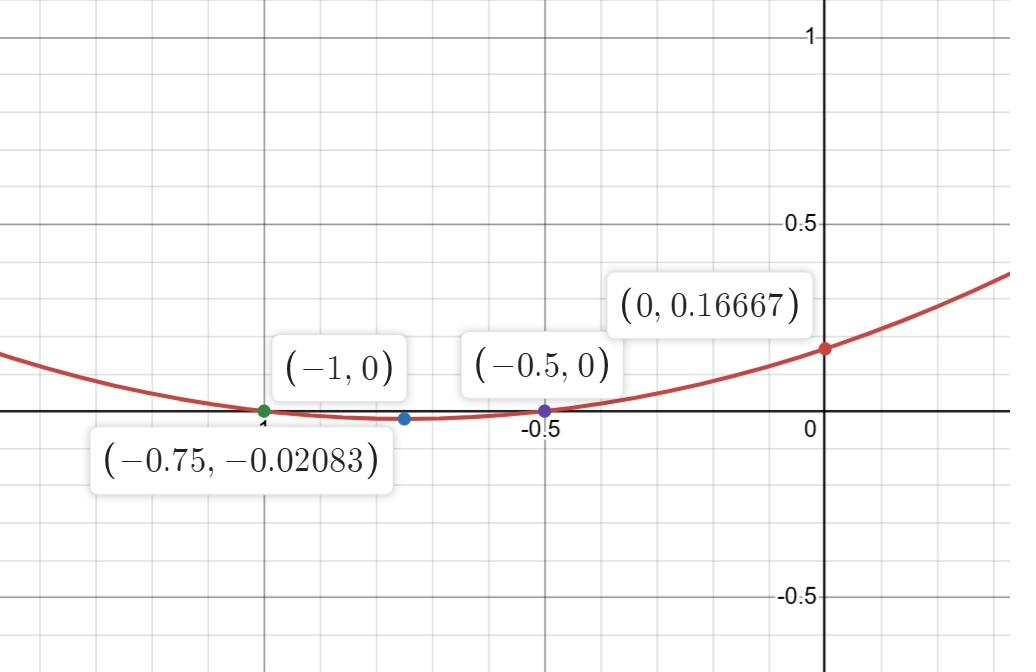
\includegraphics[width=0.80\textwidth]{bilder/Quadratische_kurve2}
  \caption{The parabola $f(x) = \tfrac{1}{6}(2x^2+3x+1)$ in the neighborhood of the
    vertex. Shown are the four geometrically distinguished
    points: the vertex $(-\tfrac{3}{4},\,-\tfrac{1}{48})$, the root
    $(-1,\,0)$, the second intersection with the $x$-axis $(-\tfrac{1}{2},\,0)$,
    and the $y$-intercept $(0,\,\tfrac{1}{6})$. The vertex provides
    the shift parameter $\beta = -\tfrac{3}{4}$ of the height function,
    while the root $(-1,\,0)$ represents the precursor point of the Euclidean
    distance sequence.}
  \label{fig:parabel_scheitel}
\end{figure}

This yields the height component of the conical helix in the form


\[
z(\theta)
= -\frac{3}{4} + \frac{3}{\pi}\,\theta,
\]


which geometrically encodes both the location of the vertex of the quadratic sequence and the
arithmetic periodicity modulo $6$. The function
$z(\theta)$ thus arises directly from the structure of the sequence
$k(n)$, without requiring an intermediate construction via the Archimedean spiral.

% ─────────────────────────────────────────────────────────────────────────────
\section{Generalization: The Construction Schema for Arbitrary Functions}
% ─────────────────────────────────────────────────────────────────────────────

The derivation developed in the preceding section possesses a
remarkable structural property: At its core, it is independent
of the specific form of the initial function $f(x)$. The decomposition into
a radial component $r(\theta)$, which determines the winding character,
and an axial component $z(\theta)$, which encodes the height progression, applies
equally to any continuous, monotonically increasing function. This section
formulates the general construction schema and shows that the present
work can be understood as a model solution for an entire class of helix constructions.

\subsection{The General Parametrization Schema}

\begin{definition}[Function-Helix]\label{def:funktionshelix}
Let $f: \mathbb{R}_{>0} \to \mathbb{R}_{>0}$ be a continuous function,
$T > 0$ a freely choosable revolution period, and $\beta \in \mathbb{R}$
a reference value. The associated \emph{function-helix} is the
space curve
\begin{equation}
\label{eq:allg_helix}
\gamma(\theta)
=
\begin{pmatrix}
f\!\left(\dfrac{T}{2\pi}\,\theta\right)\cos\theta\\[8pt]
f\!\left(\dfrac{T}{2\pi}\,\theta\right)\sin\theta\\[8pt]
\beta + \dfrac{T}{2\pi}\,\theta
\end{pmatrix},
\qquad \theta \geq 0.
\end{equation}
\end{definition}

The parametrization~\eqref{eq:allg_helix} contains three structurally
independent constituents, each contributing a distinct
geometric effect.

The \textbf{radial component} $r(\theta) = f\!\bigl(\tfrac{T}{2\pi}\theta\bigr)$
completely determines the type of the generating spiral in the $xy$-plane.
The function $f$ specifies how rapidly the distance from the $z$-axis
increases with the rotation angle $\theta$. Each choice of $f$ corresponds to a
classifiable spiral type.

The \textbf{axial component} $z(\theta) = \beta + \alpha\theta$ with
$\alpha = T/(2\pi)$ is, by contrast, identically structured for all functions $f$.
It is an affine-linear function of $\theta$ whose slope
$\alpha$ depends solely on the chosen revolution period $T$.
The choice $T = 6$ reproduces exactly the slope $\alpha = 3/\pi$ of the
conical helix. This linearity is not a peculiarity of the quadratic
initial function, but a universal consequence of the requirement for
constant height gain per revolution.

The \textbf{shift parameter} $\beta$ anchors the curve at the
distinguished reference point of $f$ -- the vertex for a
parabola, the inflection point for a cubic, the root for a
polynomial with sign-changing derivative. It ensures that
$\theta = 0$ is geometrically meaningful.

\subsection{The Distinguished Role of the Parabola}

Within the class described by Definition~\ref{def:funktionshelix},
the parabola $f(x) = (6/\pi^2)\cdot x$ occupies a
distinguished position. It is the \emph{only} function for which
the condition

\[
\frac{dz}{dr} = \frac{dz/d\theta}{dr/d\theta} = \text{const}
\]

is satisfied. Since $r(\theta) = (6/\pi^2)\theta$ is linear in $\theta$ --
just as $z(\theta)$ is -- their quotient is constant:

\[
\frac{dz}{dr}
= \frac{3/\pi}{6/\pi^2}
= \frac{\pi}{2}.
\]

This constancy means geometrically that the helix lies on a
\emph{right circular cone}. For all other functions $f$, the quantity
$dr/d\theta$ varies with $\theta$, so that the quotient $dz/dr$ becomes position-dependent
and the curve lies on a curved surface of revolution, not
on a cone.

\subsection{Classification by Spiral Type}

Depending on the choice of function $f$, qualitatively different
helix types arise, distinguished by their asymptotic growth behavior and
the associated surface of revolution. The following table
summarizes the principal cases, each with period $T = 6$
and $\alpha = 3/\pi$:

\begin{table}[H]
\centering
\caption{Classification of function-helices by choice of the
radial function $f(x)$ at fixed period $T = 6$.
The axial component $z(\theta) = \beta + (3/\pi)\theta$ is
structurally identical for all cases; only $\beta$ and $f$ vary.}
\renewcommand{\arraystretch}{1.4}
\begin{tabular}{llll}
\toprule
$f(x)$ & Spiral type & Surface of revolution & $\beta$ \\
\midrule
$\dfrac{6}{\pi^2}\,x$\quad (Archimedean)
  & Archimedean, $r \sim \theta$
  & Right circular cone $z \sim r$
  & $-\tfrac{3}{4}$ \\[6pt]
$x^{1/3}$
  & Fermat spiral, $r \sim \theta^{1/3}$
  & $z \sim r^3$
  & $0$ \\[4pt]
$\sqrt{x}$
  & Square-root spiral, $r \sim \theta^{1/2}$
  & $z \sim r^2$ (paraboloid)
  & $0$ \\[4pt]
$\ln x$
  & Logarithmic spiral
  & $z \sim e^r$
  & $0$ \\[4pt]
$x^2$
  & Quadratic spiral, $r \sim \theta^2$
  & $z \sim r^{1/2}$
  & $0$ \\
\bottomrule
\end{tabular}
\end{table}

\begin{remark}[Universality of the Height Function]
The table illustrates the central structural finding: The
height function $z(\theta) = \beta + (3/\pi)\theta$ is \emph{identical} for all
listed helix types -- apart from the scalar
shift parameter $\beta$. It is not specific to the
quadratic sequence, but a universal affine-linear function
that follows exclusively from the requirement of a constant slope
$\Delta z / \Delta\theta = T/(2\pi)$. What distinguishes the present
construction from other helices is not the
height function itself, but the provenance of its parameters: $\alpha$
and $\beta$, which are derived from the intrinsic arithmetic structure of the sequence $k(n)$. It is precisely this
arithmetic anchoring that makes the conical helix a mathematically
privileged object within the family described by
Definition~\ref{def:funktionshelix}.
\end{remark}

\subsection{The Construction Schema as a Model Solution}

The foregoing analysis allows us to formulate the procedure developed in this chapter
as a general construction schema that
can be transferred to arbitrary initial functions. The schema
consists of three mutually independent steps.

\textbf{Step 1 -- Choice of function and reference point.}
Let a continuous function $f(x)$ be given. The reference point $x_0$ is
the distinguished point of $f$ -- vertex, inflection point, or
root -- and yields the shift parameter $\beta = -\alpha\,\varphi$,
where $\varphi$ is the phase offset of the angular coupling $\theta_{x_0} = 0$.

\textbf{Step 2 -- Choice of the revolution period $T$.}
The period $T$ specifies which increment in $x$ corresponds to a complete
revolution. It determines the slope $\alpha = T/(2\pi)$
of the height function and the linear coupling $x(\theta) = (T/2\pi)\,\theta$.
For the quadratic sequence $k(n)$, the value $T = 6$ is distinguished by the
congruence structure $n \equiv 1, 5 \pmod{6}$.

\textbf{Step 3 -- Parametrization of the helix.}
The complete curve follows immediately from
Equation~\eqref{eq:allg_helix}. The winding character is determined by $f$,
the height progression by $T$, and the spatial position by $\beta$.
No further construction assumptions are required.

\begin{remark}[Geometric Intuition]
The schema can be understood intuitively as follows: The curve $y = f(x)$ in the
plane is conceived as a flexible strip that is wound around the
$z$-axis -- similar to a strip of paper rolled into a
spiral. The slope during winding is $\alpha$, the
radius at each height follows from the function value $f(x(\theta))$, and
the starting point of the winding corresponds to $\beta$. The result is always
a well-parametrized space curve whose geometric properties
are completely determined by $f$, $T$, and $\beta$.
\end{remark}
